Die Abbildung \ref{fig:TestingPyramide} ist ein Vergleich zwischen den verschiedenen Testtypen zueinander.
Es werden fünf Testtypen miteinander verglichen, die in den nächsten Kapiteln beschrieben werden. 
Die Kategorien, in denen die Testtypen miteinander verglichen werden, sind:
\begin{itemize}
    \item Anzahl an Tests
    \item Komplexität
    \item Zerbrechlichkeit
    \item Wartungskosten
    \item Laufzeit
    \item Zeit um den Fehler zu lokalisieren
\end{itemize} 
Die Farben in der Pyramide symbolisieren die Priorisierung jedes einzelnen Testtypes.
Laut der Pyramide sollen zum Beispiel Unittests vor Integrationtests priorisiert werden.
D.h. die Integrationtests testen keine Funktionalitäten, die mit Unittests abgedect werden können. 


\begin{figure}[H]
    \centering
    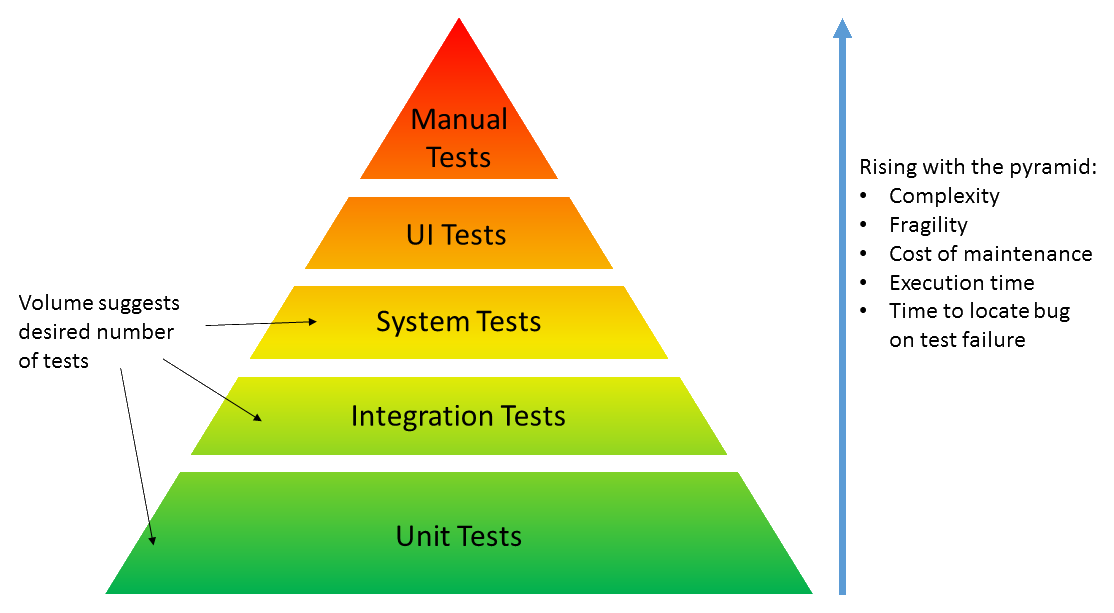
\includegraphics[width=1\textwidth]{Images/test_pyramid.png}
    \caption[Testing Pyramide]{Caption written below figure \footnotemark}
    \label{fig:TestingPyramide}
\end{figure}
\footnotetext{https://www.cqse.eu/de/news/blog/junit3-migration/}